% Anonymized draft for Journal of Mathematical Philosophy (initial submission).
% Open formatting OK at submission; switch to JMP template after acceptance.
% Polish pass: classification-first; three-layer separation; no new mathematics.
\documentclass[11pt,a4paper]{article}

\usepackage[margin=1.1in]{geometry}
\usepackage{microtype}
\usepackage{amsmath,amssymb,amsthm}
\usepackage{mathtools}
\usepackage{tikz}
\usetikzlibrary{arrows.meta,positioning,calc,fit}
\usepackage[hidelinks]{hyperref}
\usepackage{enumitem}
\usepackage{booktabs}

\newtheorem{theorem}{Theorem}[section]
\newtheorem{proposition}[theorem]{Proposition}
\newtheorem{lemma}[theorem]{Lemma}
\newtheorem{corollary}[theorem]{Corollary}
\newtheorem{definition}[theorem]{Definition}
\theoremstyle{remark}
\newtheorem{remark}[theorem]{Remark}
\newtheorem{interpretation}[theorem]{Interpretation}
\newtheorem*{statusopen}{Open}
\newtheorem*{statusrefused}{Refused}
\newtheorem*{statusphil}{Philosophical}

\newcommand{\Fund}{\mathsf{Fund}}
\newcommand{\Bool}{\mathsf{Bool}}
\newcommand{\comp}{\circ}
\newcommand{\Ztwo}{\mathbb{Z}/2\mathbb{Z}}
\newcommand{\act}{a}

\title{Classification of Self-Actions and the Unique Involutive Survivor}
\author{} % anonymized for double-anonymous review
\date{}

\begin{document}
\maketitle

\begin{abstract}
We classify self-actions $a:\alpha\to\alpha$ by local orbit shape. Rest,
asymmetric step, and erasure each meet a formal obstruction in the ambient
of pointed symmetric steps; the surviving shape is the fixed-point-free
two-cycle. That survivor is characterised by a universal property:
$(\Bool,\neg)$ is initial among pointed unoriented acts, and every
fundamental act reads as negation. From fundamentality we obtain a
Lawvere-style seal (no point-surjective self-reading), an $\omega$-ladder
of namers, and---after transferring losslessness to forward microsteps by
two-bounce factorisation---registration, capacity, and a single
$\Ztwo$-underdetermination with three faces. Canonicity of the two-bounce
pair fails; channel \emph{swap} nevertheless covers step reversal. Content
gauges are separated from packaging gauges so that factorisation
non-uniqueness does not inflate the dictionary $\Ztwo$. The development
is machine-checked in Lean~4 (no Mathlib, no $\mathtt{sorry}$). Physical
readings appear only in a dictionary layer of certificates.
\end{abstract}

\noindent\textbf{Keywords:}
classification; involution; universal property; Lawvere diagonal;
underdetermination; gauge; machine-checked mathematics.

\section{Introduction}
\label{sec:intro}

The central contribution of this paper is an \emph{eliminative
classification of self-actions}. Given $a:\alpha\to\alpha$, the local
possibilities at a state are rest, two-cycle, asymmetric step, and---as a
pairwise defect---erasure. In a precisely specified ambient, every shape
except one encounters an obstruction. The survivor is the live two-cycle.
Negation on $\Bool$ is not assumed at the outset; it is the unique object
(up to label swap) satisfying the universal property of that survivor.

The formal development then follows a fixed dependency:
\begin{center}
classification $\rightarrow$
fundamentality $\rightarrow$
seal $\rightarrow$
ladder $\rightarrow$
registration $\rightarrow$
archive $\rightarrow$
capacity $\rightarrow$
arrow $\rightarrow$
interpretations.
\end{center}
Each arrow is a theorem or a defined interface; philosophical commentary
is postponed until the supporting machinery is in place.

\paragraph{Method and layers.}
The text maintains three layers.
\begin{enumerate}[label=(\arabic*),leftmargin=*]
\item \textbf{Formal mathematics} --- definitions, theorems, proofs.
\item \textbf{Philosophical interpretation} --- what the mathematics
suggests, marked as such.
\item \textbf{Dictionary} --- optional physical or contemplative
identifications, admitted only by certificate.
\end{enumerate}
Claims are tagged by status: proved, corollary, interpretation, open,
refused, or philosophical residue. The companion Lean~4 corpus (no
Mathlib, no $\mathtt{sorry}$) supplies declaration names; this paper is
self-contained at the level of statements.

\paragraph{Roadmap.}
Section~\ref{sec:arch} gives the architecture.
Sections~\ref{sec:class}--\ref{sec:fund} carry out the classification and
the universal characterisation of the survivor.
Sections~\ref{sec:seal}--\ref{sec:ladder} obtain seal and ladder.
Sections~\ref{sec:reg}--\ref{sec:arrow} transfer losslessness, record
registration and capacity, and identify the arrow with address.
Section~\ref{sec:z2} states the single $\Ztwo$ and the gauge demarcation.
Section~\ref{sec:dict} confines dictionary readings.
Section~\ref{sec:status} collects open, refused, and philosophical items.
Section~\ref{sec:concl} concludes.


\section{Architecture}
\label{sec:arch}

The companion corpus is stratified into three layers with downward-only
imports (Figure~\ref{fig:layers}).

\begin{figure}[ht]
\centering
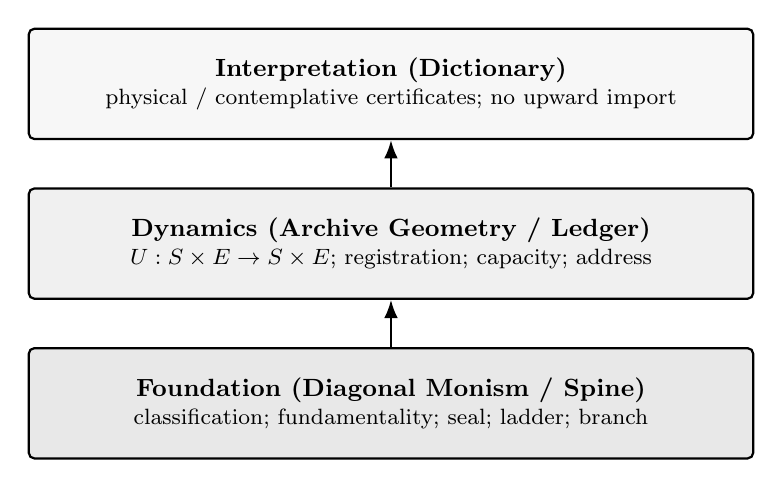
\begin{tikzpicture}[
  font=\small,
  layer/.style={draw, thick, rounded corners=2pt, minimum width=92mm,
    minimum height=14mm, align=center, inner sep=4pt},
  arr/.style={-{Latex}, thick}
]
\node[layer, fill=gray!6] (dict) {%
  \textbf{Interpretation (Dictionary)}\\[-1pt]
  {\footnotesize physical / contemplative certificates; no upward import}};
\node[layer, fill=gray!12, below=6mm of dict] (led) {%
  \textbf{Dynamics (Archive Geometry / Ledger)}\\[-1pt]
  {\footnotesize $U:S\times E\to S\times E$; registration; capacity; address}};
\node[layer, fill=gray!18, below=6mm of led] (sp) {%
  \textbf{Foundation (Diagonal Monism / Spine)}\\[-1pt]
  {\footnotesize classification; fundamentality; seal; ladder; branch}};
\draw[arr] (sp) -- (led);
\draw[arr] (led) -- (dict);
\end{tikzpicture}
\caption{Three-layer architecture. Arrows indicate permitted dependence
(foundation supports dynamics; dynamics support interpretation). The
figure orients the reader; it proves nothing.}
\label{fig:layers}
\end{figure}

\noindent
Within the foundation, the dependency is
classification~$\to$~fundamentality~$\to$~seal~$\to$~ladder.
The dynamics layer imports losslessness along an interface
(registration via two-bounce), realises archive and capacity on the
ladder carrier, and exports address as the arrow reading. The dictionary
layer consumes those exports; it does not feed them.


\section{Classification of self-actions}
\label{sec:class}

\begin{definition}[Arena data]
\label{def:arena}
Fix a type $\alpha$ and a map $a:\alpha\to\alpha$. Write
\[
  \mathsf{Step}(a)(x,y)\ :\Leftrightarrow\ y=a(x).
\]
Call $a$ a \emph{symmetric step} when $\mathsf{Step}(a)$ is a symmetric
relation; equivalently, $a\comp a=\mathrm{id}$. Call $a$ \emph{live}
when $\forall x.\, a(x)\neq x$. Call $a$ \emph{lossless} when $a$ is
injective. Call $a$ \emph{erasing} when distinct states share a
successor.
\end{definition}

\begin{theorem}[Pointwise classification]
\label{thm:class}
For decidable equality on $\alpha$, at each $z$ exactly one of the
following holds: (i)~rest ($a(z)=z$), with all iterates stagnant;
(ii)~two-cycle at $z$ ($a(z)\neq z$ and $a(a(z))=z$), with every iterate
equal to $z$ or $a(z)$; (iii)~asymmetric step at $z$ ($a(a(z))\neq z$).
The three cases are pairwise incompatible. Erasure is diagnosed
separately as a pairwise defect of losslessness.
\end{theorem}

\begin{remark}[Status]
Theorem~\ref{thm:class} is proved. It is the eliminative engine of the
paper: subsequent sections impose ambient constraints under which (i)
and (iii), and erasure, are excluded as candidates for fundamentality.
\end{remark}

Symmetric step is the ambient equation used below. It jointly excludes
asymmetric arrow (case~(iii) globally) and, by the next corollary,
erasure.

\begin{proposition}[In-arena losslessness]
\label{prop:no-erase}
If $a$ is a symmetric step, then $a$ is not erasing.
\end{proposition}

\begin{remark}[Status]
Corollary of Definition~\ref{def:arena} (involution $\Rightarrow$
injectivity). Not an independent creed.
\end{remark}

\begin{interpretation}
\label{int:ambient}
The choice of symmetric step as ambient is a modelling decision: it
bans smuggled time (asymmetric step) and smuggled loss (erasure) by one
equation. Whether that ambient is the ``right'' one for fundamentality
is philosophical residue (Section~\ref{sec:status}), not a theorem.
\end{interpretation}


\section{Fundamentality as universal property}
\label{sec:fund}

\begin{definition}[Pointed unoriented acts]
\label{def:ambient}
Objects are triples $(\alpha,a,z)$ with $a$ a symmetric step and
$z:\alpha$ a seed. Morphisms are pointed equivariant maps.
\end{definition}

Rest is incompatible with liveness. Asymmetric step is incompatible with
symmetric step. Erasure is incompatible with Proposition~\ref{prop:no-erase}.
Relative to Definition~\ref{def:ambient} and liveness, the only remaining
pointwise shape is the live two-cycle.

\begin{theorem}[Canon / initiality]
\label{thm:canon}
In the ambient of pointed unoriented acts, $(\Bool,\neg,\mathsf{true})$
is initial. An act is \emph{fundamental} precisely when it is live,
symmetric, and generated from a seed by the two-cycle reading; every
fundamental reads as $\neg$; any two fundamentals correspond uniquely
up to the pointed reading.
\end{theorem}

\begin{remark}[Status]
Proved. Negation is the unique (up to label swap) object satisfying the
universal property of the live two-cycle in this ambient---the survivor
of the classification, not a primitive assumption.
\end{remark}

\begin{interpretation}
\label{int:fund}
``The fundamental'' names that initial object after uniqueness.
Excluded fixed point (``void'') is liveness restated. Label swap of the
two poles is a content gauge: exported readings mention it; see
Section~\ref{sec:z2}.
\end{interpretation}


\section{Seal}
\label{sec:seal}

Dependence: Theorem~\ref{thm:canon} (liveness of fundamentals).

\begin{theorem}[Seal on a fundamental]
\label{thm:seal}
Let $a$ be live. No map $f:A\to (A\to\Bool)$ is point-surjective: the
diagonal dodge $x\mapsto \neg(f\,x\,x)$ is missed. Specialising to
fundamental acts, every self-reading admits an escape.
\end{theorem}

\begin{theorem}[Corpus-grain incompleteness]
\label{thm:corpus}
No self-reading of the formal corpus is universal for the predicates of
its own level: names are outnumbered by predicates, and any completed
self-portrait lags. Completeness-in-the-limit is a fair-schedule
\emph{policy}, not a theorem that the corpus catches itself.
\end{theorem}

\begin{remark}[Status]
Theorems~\ref{thm:seal}--\ref{thm:corpus} are proved (Lawvere-style;
no arithmetisation). Host-logic incompleteness and G\"odel coding of the
corpus text are \emph{refused} (Section~\ref{sec:status}).
\end{remark}


\section{Ladder}
\label{sec:ladder}

Dependence: Theorem~\ref{thm:seal} (named escapes).

\begin{definition}[Naming extension and ladder]
\label{def:ladder}
A \emph{naming extension} adjoins a name for an unrepresented escape. The
committed ladder sets level~$0$ to the fundamental carrier and each
successor to an option type adjoining a namer for the previous dodge.
\end{definition}

\begin{theorem}[Ladder properties]
\label{thm:ladder}
History embeds injectively and conservatively along the ladder; no level
is exhausted by its predecessor; underdetermination persists at every
level. Ascent is forced; choice of which escape is named is free.
\end{theorem}

\begin{remark}[Status]
Proved in the foundation layer. Duration, as used below, means the
order-type of this self-escape sequence.
\end{remark}

\begin{interpretation}
\label{int:ladder}
The pattern ``forced relation, free absolute''---forced ascent, free
direction---reappears for channel labels in Section~\ref{sec:reg}.
\end{interpretation}


\section{Registration: transferring losslessness}
\label{sec:reg}

Spine acts are involutions. A ledger microstep is a forward map
$U:S\times E\to S\times E$. The interface demand is that global
injectivity of $U$ import Proposition~\ref{prop:no-erase}.

\begin{definition}[Two-bounce factorisation]
\label{def:twobounce}
A \emph{two-bounce factorisation} of $U:\alpha\to\alpha$ is a pair of
involutions $(\phi,\sigma)$ with $U=\sigma\comp\phi$ pointwise.
\end{definition}

\begin{theorem}[Converse]
\label{thm:converse}
If $U$ admits a two-bounce factorisation, then $U$ is lossless. On a
product carrier this is ledger injectivity.
\end{theorem}

\begin{theorem}[Existence on finite carriers]
\label{thm:exists}
Every injective $U:\mathrm{Fin}\,n\to\mathrm{Fin}\,n$ admits a
two-bounce factorisation. The construction is cycle-wise reflection at a
least-value basepoint, with $\sigma:=U\comp\phi$.
\end{theorem}

\begin{remark}[Status]
Theorems~\ref{thm:converse}--\ref{thm:exists} are proved. On finite
carriers, injectivity and two-bounce form coincide. Special cases
(involutions as $U\comp\mathrm{id}$; Boolean injections; swap step) are
included.
\end{remark}

\begin{theorem}[Registration shape]
\label{thm:reg}
Under joint injectivity, a system merge writes a record in the
environment (registration). Minimal merge alphabet size is $2$, matching
$|\Fund|$.
\end{theorem}

\begin{remark}[Status]
Proved in the dynamics layer, using the injectivity interface above.
\end{remark}

\subsection{Canonicity of the factor pair}

\begin{theorem}[Canonicity fails]
\label{thm:canonfail}
There exist an injective $U:\Bool\to\Bool$ and two two-bounce
factorisations that disagree on $\phi$ (equivalently: $\neg$ factors as
both $\neg\comp\mathrm{id}$ and $\mathrm{id}\comp\neg$).
Moreover, on $\mathrm{Fin}\,3$ two reflection-axis factorisations of a
$3$-cycle disagree and are not related by bounce-swap
$(\phi,\sigma)\mapsto(\sigma,\phi)$.
\end{theorem}

\begin{remark}[Status]
Proved negative. The absolute position of the factor pair is a
\emph{packaging} gauge (Section~\ref{sec:z2}): the ledger consumes $U$,
never $(\phi,\sigma)$.
\end{remark}

\begin{theorem}[Channel-swap is reversal]
\label{thm:swap}
Let $U=\sigma\comp\phi$ with $\phi,\sigma$ involutions. Then
$\phi\comp\sigma$ is a two-sided inverse of $U$, and $(\sigma,\phi)$ is
a two-bounce presentation of that reverse step. The construction is
independent of which factorisation of $U$ was chosen.
\end{theorem}

\begin{proof}[Proof sketch]
From $U=\sigma\comp\phi$ and the involution equations,
$\phi(\sigma(U(x)))=\phi(\sigma(\sigma(\phi(x))))=\phi(\phi(x))=x$ and
$U(\phi(\sigma(x)))=\sigma(\phi(\phi(\sigma(x))))=\sigma(\sigma(x))=x$.
The swapped pair $(\sigma,\phi)$ presents the reverse step. Uniqueness
of $(\phi,\sigma)$ is not used.
\end{proof}

\begin{figure}[ht]
\centering
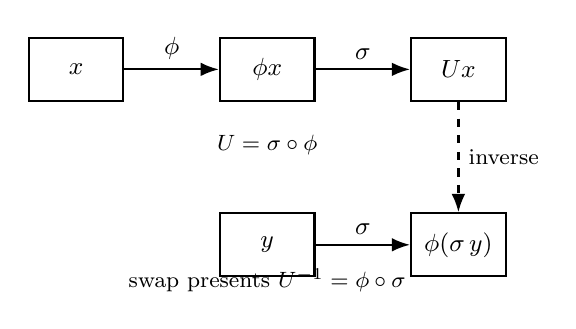
\begin{tikzpicture}[
  font=\small,
  m/.style={draw, thick, minimum width=12mm, minimum height=8mm, align=center},
  arr/.style={-{Latex}, thick}
]
\node[m] (x) {$x$};
\node[m, right=12mm of x] (phix) {$\phi x$};
\node[m, right=12mm of phix] (ux) {$Ux$};
\draw[arr] (x) -- node[above]{$\phi$} (phix);
\draw[arr] (phix) -- node[above]{$\sigma$} (ux);
\node[m, below=14mm of ux] (rev) {$\phi(\sigma\,y)$};
\node[m, left=12mm of rev] (y) {$y$};
\draw[arr] (y) -- node[above]{$\sigma$} (rev);
\draw[arr, dashed] (ux) -- node[right]{\footnotesize inverse} (rev);
\node[below=3mm of phix, align=center, font=\footnotesize]
  {$U=\sigma\comp\phi$};
\node[below=20mm of phix, align=center, font=\footnotesize]
  {swap presents $U^{-1}=\phi\comp\sigma$};
\end{tikzpicture}
\caption{Two-bounce presentation and swap. Pair labels are conventional;
exchange covers reversal (Theorem~\ref{thm:swap}).}
\label{fig:bounce}
\end{figure}

\begin{interpretation}
\label{int:mirrors}
In the dihedral picture, a rotation fixes the angle between mirrors, not
their absolute position. Theorem~\ref{thm:canonfail} is that fact on
finite carriers; Theorem~\ref{thm:swap} promotes the exchange.
\end{interpretation}


\section{Archive and capacity}
\label{sec:archive}

Dependence: ladder carrier (Section~\ref{sec:ladder}) as environment;
registration (Theorem~\ref{thm:reg}).

\begin{theorem}[Archive and capacity]
\label{thm:caps}
Taking the environment at horizon $T$ to be the ladder carrier at
level~$T$, the committed capacity schedule satisfies
$|\mathrm{caps}\,T|=2^{T+2}$. Joint injectivity, merge, muting, and
confinement imply the combinatorial bound $K^{T}\le|\mathrm{caps}\,T|$;
at $K=2$ the committed ladder is eternally alive by arithmetic.
\end{theorem}

\begin{remark}[Status]
Proved in the dynamics layer. Continuum area or continuum entropy
identifications are refused.
\end{remark}


\section{Arrow as address}
\label{sec:arrow}

Dependence: registration and archive growth.

\begin{theorem}[Arrow reading]
\label{thm:arrow}
The dynamical arrow---archive ascent under registration---is identified
with address valued in $\{\mathsf{fwd},\mathsf{rev}\}$. Tick identification
(naming tick with microtick) holds for the classified fragment of
uniform free archives up to record gauge; periodic fund-exempt dynamics
and swap necessity are part of that classification.
\end{theorem}

\begin{remark}[Status]
Proved as a classified package in the dynamics layer. Record gauge is
packaging: exported only inside ``up to record gauge'' clauses.
\end{remark}


\section{One underdetermination and gauges}
\label{sec:z2}

Dependence: pole swap from Theorem~\ref{thm:canon}; address from
Theorem~\ref{thm:arrow}; channel from Definition~\ref{def:twobounce} and
Theorem~\ref{thm:swap}.

\begin{theorem}[One $\Ztwo$, three faces]
\label{thm:z2}
There is a single two-element underdetermination with three named
involutive projections:
\begin{center}
pole swap \quad$\cong$\quad
address $\{\mathsf{fwd},\mathsf{rev}\}$ \quad$\cong$\quad
channel $\{\varphi,\sigma\}$.
\end{center}
Each projection is an involution on a common $\Ztwo$ carrier.
\end{theorem}

\begin{figure}[ht]
\centering
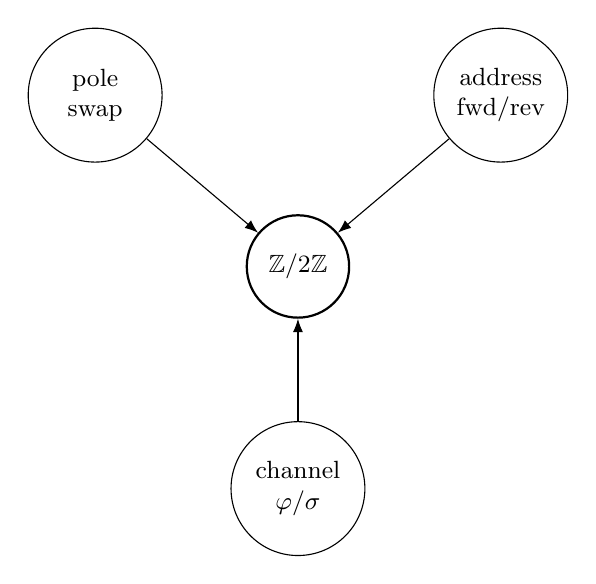
\begin{tikzpicture}[
  font=\small,
  face/.style={draw, circle, minimum size=17mm, align=center, inner sep=1pt},
  hub/.style={draw, thick, circle, minimum size=13mm, align=center}
]
\node[hub] (z) {$\Ztwo$};
\node[face, above left=11mm and 15mm of z] (p) {pole\\swap};
\node[face, above right=11mm and 15mm of z] (a) {address\\fwd/rev};
\node[face, below=13mm of z] (c) {channel\\$\varphi/\sigma$};
\draw[-{Latex}] (p) -- (z);
\draw[-{Latex}] (a) -- (z);
\draw[-{Latex}] (c) -- (z);
\end{tikzpicture}
\caption{Three faces of one underdetermination (Theorem~\ref{thm:z2}).
Faces are presentations; the group is stated once.}
\label{fig:z2}
\end{figure}

\begin{definition}[Content vs packaging]
\label{def:gauge}
A gauge is \emph{content} when some exported statement mentions the
choice. A gauge is \emph{packaging} when the choice is quotiented before
downstream consumption.
\end{definition}

\begin{center}
\begin{tabular}{@{}lll@{}}
\toprule
Gauge & Locus & Class \\
\midrule
Label / pole swap & Theorem~\ref{thm:canon} & content \\
Address fwd/rev & Theorem~\ref{thm:arrow} & content \\
Channel swap & Theorem~\ref{thm:swap} & content \\
Record gauge per tick & Theorem~\ref{thm:arrow} & packaging \\
Factorisation gauge per step & Theorems~\ref{thm:exists}--\ref{thm:canonfail}
  & packaging \\
\bottomrule
\end{tabular}
\end{center}

\begin{remark}[Status]
Theorem~\ref{thm:z2} and Definition~\ref{def:gauge} keep one dictionary
$\Ztwo$: factorisation non-uniqueness (Theorem~\ref{thm:canonfail}) is
packaging; channel \emph{labels} are conventional; channel \emph{swap}
is content.
\end{remark}


\section{Dictionary interpretations}
\label{sec:dict}

\begin{interpretation}
\label{int:dict}
Dictionary entries are optional certificates that a physical or
contemplative model realises kernel symmetries (for example, swap as
negation, dissipation as registration). They do not derive continuum
spacetimes or observational numbers from $\Bool$.
\end{interpretation}

\begin{remark}[Status]
Layer~3 only. No theorem in Sections~\ref{sec:class}--\ref{sec:z2}
depends on a dictionary certificate.
\end{remark}


\section{Open, refused, and philosophical}
\label{sec:status}

\begin{statusopen}
Continuum Lorentzian structure and boosts (no continuous one-parameter
subgroup from a single $\Ztwo$); Mathlib-level sheaf assembly beyond
landed stalk fragments; recombination budget versus ultrametric
obstruction; deeper alphabet-lift optional once Fin interfaces close.
\end{statusopen}

\begin{statusrefused}
Premise-free global laws of time; continuum Einstein equations as
theorems of this corpus; host-logic incompleteness; G\"odel
arithmetisation of the formal text; experiential or qualia claims;
derivation of the world from $\Bool$ alone.
\end{statusrefused}

\begin{statusphil}
Facticity of liveness; adequacy of the pointed unoriented ambient
(Interpretation~\ref{int:ambient}); which face of the $\Ztwo$ is treated
as free in applications.
\end{statusphil}


\section{Conclusion}
\label{sec:concl}

The classification theorem restricts self-actions to the live two-cycle
under the stated ambient. Fundamentality is the universal property of
that survivor: the unique object is $(\Bool,\neg)$ up to label swap.
Seal, ladder, registration (via two-bounce), archive capacity, and arrow
as address follow in dependency order. One $\Ztwo$ is stated once; content
and packaging gauges prevent factorisation non-uniqueness from counting
as a second underdetermination. Philosophical and dictionary claims are
confined to marked layers and to Section~\ref{sec:status}.

\section*{Formal companion}
\label{sec:companion}

Representative declarations:
\texttt{classification\_at},
\texttt{canon\_initial},
\texttt{symmetric\_excludes\_erase},
\texttt{seal\_on\_fundamental},
\texttt{corpus\_not\_universal},
\texttt{one\_Z2\_three\_faces},
\texttt{factor\_fin},
\texttt{canonicity\_fails},
\texttt{channel\_swap\_is\_reversal},
\texttt{registration},
\texttt{caps\_eq},
\texttt{tick\_identification}.
Axiom footprints are audited per declaration.

\begin{thebibliography}{99}

\bibitem{lawvere}
F.~W.~Lawvere.
\newblock Diagonal arguments and Cartesian closed categories.
\newblock \emph{Category Theory, Homology Theory and Their Applications},
  1969.

\bibitem{dihedral}
H.~S.~M.~Coxeter.
\newblock \emph{Regular Polytopes}.
\newblock Dover, 1973.
\newblock (Dihedral factorisation of rotations as products of reflections.)

\bibitem{bool}
G.~Boole.
\newblock \emph{An Investigation of the Laws of Thought}.
\newblock 1854.

\bibitem{quine}
W.~V.~Quine.
\newblock Ontological relativity.
\newblock In \emph{Ontological Relativity and Other Essays}, Columbia,
  1969.

\end{thebibliography}

\end{document}
